\chapter{Evaluation and Analysis}

In the first part of this chapter we briefly characterize the nature of the data set used for evaluation of the models summarized in chapters~\ref{relevant-models} and \ref{models-timing} and discuss some specifics of the implementation. In the second part we report on evaluation of models predictions, parameter fitting procedure, stability of parameters, and extensions of the models. The experiments were performed using data of real students from the adaptive system Outline~Maps. In the last part we summarize results from further analysis of the models.

\section{Data Set}

For evaluation of our models, we used data from the adaptive educational system \url{slepemapy.cz}. The data set contains more than 10~million answers from tens of thousands of unique users, mostly Czech students~\cite{Papousek2015}. In our experiments, we filtered the data set so that it contains only answers of students who practiced at least 50 items, furthermore the places that were answered by less then 100 students were removed. Note that we usually run our experiments only on a portion of the whole data set.

Considering the system is adaptive, the selection of questions is based on student's knowledge, instead of being statically programmed by an expert. The system has target probability 75\%, i.e. the questions which are expected to be too hard or too easy for the student are penalized by a \textit{scoring function}. The scoring function is responsible for the selection of question to be practiced~\cite{Stanislav2015thesis}. The adaptability of the system should be also taken into consideration as it might have affected the results of our analysis.

The used data set further contains very different students with distinct prior knowledge, some students are still in school and practice geography in classes, other students already finished school and want to revive their forgotten knowledge (this is further analyzed in chapter~\ref{further-analysis}). There are also huge differences between continents, regions and other types of places, all of which may vary in the easiness of learning, some may be harder for the majority of Czech students to retain and are thus forgotten faster (e.g. some small African country that most students never heard of).

\section{Toolchain}

The models were implemented in Python programming language. Experiments were performed in the Jupyter Notebook interactive environment\footnote{Jupyter Notebook is an open sourced web application for interactive computing, see~\url{https://jupyter.org/}}. Here is a list of the used libraries and modules:

\begin{itemize}
  \item SciPy, NumPy, Pandas -- numerical calculations and data analysis.
  \item Matplotlib, Seaborn, NetworkX -- data visualization.
  \item Scikit-Learn -- miscellaneous machine learning helpers.
\end{itemize}

\section{Baseline}

As a baseline we use the standard PFA model and two of its extensions. We use acronyms for all evaluated models, here is a list of the baseline models as their acronyms occur in our experiments:

\begin{itemize}
  \item \textbf{PFA} -- the original performance factor analysis which we described in chapter~\ref{pfa}. Note that our implementation doesn't consider multiple knowledge components.
  \item \textbf{PFA/E} -- a version of the original PFA model with some aspects of Elo model which we discussed in chapter~\ref{pfae}.
  \item \textbf{PFA/G} -- another version of the original PFA model with a decay factor, the characteristics of the model were outlined in chapter~\ref{pfag}.
\end{itemize}

Note that for the estimation of prior knowledge we use the Elo model briefly described in chapter~\ref{elo}. In all our models, the initial memory activation $m$ is estimated as $\theta_s - d_i$ as we explained in chapter~\ref{pfa}.

\section{Response Time}

The response time of a student may indicate student's knowledge of an item. If the student answered quickly, almost automatically, it is very likely they either know the place very well or are purely guessing, depending on the correctness of their answer. On the other hand when the response is longer, the student is probably familiar with the item and might eventually recall the correct answer. The relationship between response times and students knowledge was discusses in a related work~\cite{papouvsekanalysis}, here we perform experiments with models that reflect this phenomenon.

Figure~\ref{fig:response-times} illustrates the relationship between students' response times and correctness of answers. If the student answers suspiciously fast (response time is lower than 800 milliseconds), it usually means they are guessing. The data set suggests that the highest probability of correct performance is between 1500 and 2000 milliseconds of response time.

\begin{figure}[htbp]
  \centering
  \begin{subfigure}{.49\textwidth}
    \centering
    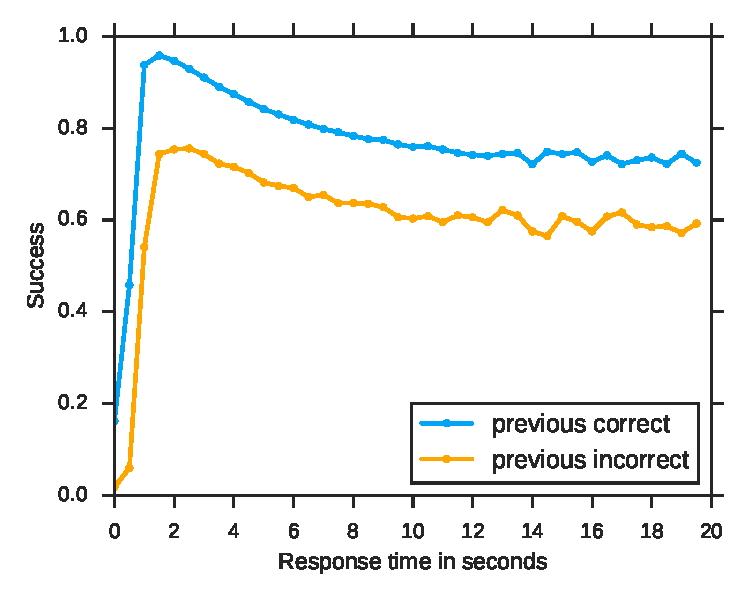
\includegraphics[width=\textwidth]{img/response-times-averaged}
    \caption{}
    \label{fig:response-times-averaged}
  \end{subfigure}
  \begin{subfigure}{.49\textwidth}
    \centering
    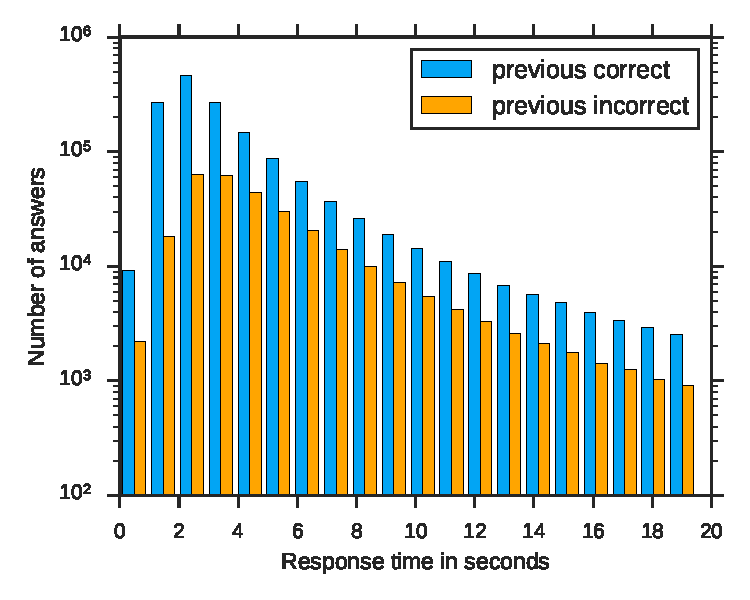
\includegraphics[width=\textwidth]{img/response-times-hist}
    \caption{}
    \label{fig:response-times-hist}
  \end{subfigure}
  \caption{Response times of students. Figure (a) shows relationship between response times and correctness of answers. Each line represent items which students answered either correctly or incorrectly in the previous trial. The data set was divided into 40 bins of equal sizes and each point is an average of correctness of answers from the corresponding bin. The number of items in each bin is depicted in figure (b) (note that the $y$-axis is logarithmically scaled).}
  \label{fig:response-times}
\end{figure}

We evaluate one model focused on improving performance by taking into account the response times of students:

\begin{itemize}
  \item \textbf{PFA/E/RT} -- an extended version of the PFA/E model which alters student's knowledge by respecting past response times. We described the model in chapter~\ref{pfart}.
\end{itemize}

Note that some places cover wider area on the map then others, i.e. a question asking a student to locate Russia has generally lower response time than a question requiring to locate Andorra since usually students have to zoom using the mouse wheel before they can respond.

\subsection{Parameters}
\label{response-parameters}

The extended PFA model has 2 parameters when we use Elo model for the estimation of prior knowledge. Thus we need to estimate $\gamma$, $\delta$ and the response time functions $r_{\mathit{succ}}$ and $r_{\mathit{fail}}$. We learned the shape of both functions from the data as indicated in Figure~\ref{fig:response-times-averaged}.

\section{Memory Decay}

In this chapter we describe parameter optimization and calibration techniques of the models focused on memory decay and forgetting. We focus on the following extensions of models:

\begin{itemize}
  \item \textbf{PFA/E/T} -- an extended version of the PFA/E model which adapts the idea of a time effect function. We described the model in chapter~\ref{pfaet}. In our analysis we examine several time effect functions formalized in chapter~\ref{time-effect-functions} including the staircase function.
  \item \textbf{PFA/G/T} -- our version of the PFA/G model which uses a time effect function instead of a decay factor. The differences were stated in chapter~\ref{pfagt}.
\end{itemize}

\subsection{Parameters}
\label{memory-parameters}

Standard PFA model has 3 global parameters when we consider only one knowledge component, that is the difficulty $\beta$ and the weight of each success $\gamma$ and failure $\delta$. In cases where we use Elo model for prior knowledge estimation, we can replace the global parameter $\beta$ with $\theta_s - d_i$ (i.e. the difference between skill of the student $s$ and difficulty of the item $i$) which leaves 2 parameters we need to estimate in the model with no time effect function.

However, a time effect function has to be selected as well. The list of functions we used in our experiments was presented in chapter~\ref{time-effect-functions}. Because all these functions have only the parameters $a$ and $c$, in the PFA/E/T model, we are required to estimate $\gamma$, $\delta$ and parameters of a chosen time effect function. In the PFA/G/T model, we need to estimate parameters of two time effect functions, $f_{\mathit{succ}}$ and $f_{\mathit{fail}}$. We were able to estimated the parameters of both models using hill climbing algorithm detailed in chapter~\ref{hill-climbing}.

In our experiments related to the staircase function formalized in chapter \ref{staircase-function}, we divided the vector $\textbf{i}$ producing 10 intervals with values between 0~seconds, 60~seconds, 90~seconds, 150~seconds, 5~minutes, 10~minutes, 30~minutes, 3~hours, 24~hours, 5~days, and more than 5~days. We picked the values so that the intervals containing the ages of last trials are easy to read and also contain sufficient amount of answers. Thus, the number of parameters to estimate is 12 including $\gamma$ and $\delta$. We learned the estimates from the data set using the adjusted gradient descent described in chapter~\ref{gradient-descent}. The fitted staircase function is illustrated in Figure~\ref{fig:learned-time-effect-function}.

\begin{figure}[htbp]
  \centering
  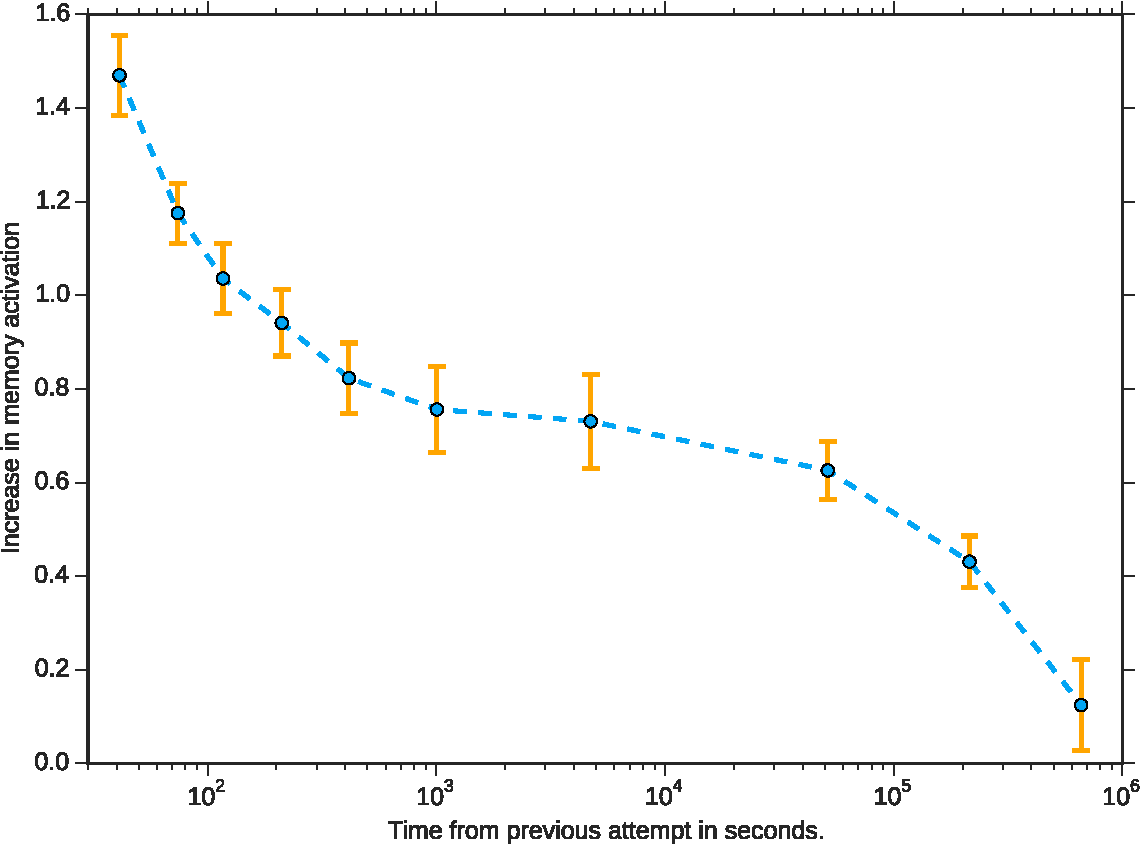
\includegraphics[width=\textwidth]{img/learned-time-effect-function}
  \caption{Time effect function as learned from the data with standard deviations. Each point represents average of 10 independent data sets containing answers of students who used the system for one week at least and answered more than 100 answers.}
  \label{fig:learned-time-effect-function}
\end{figure}

The figure shows that the parameters are rather stable (with $\gamma = 1.814 \pm 0.276$ and $\delta = 0.827 \pm 0.095$) and also that the staircase function appears to be a good choice as a time effect function. The learned values also suggest that none of the simple time effect functions' shapes fits the staircase function, although the logarithmic and power functions might be close approximations---this we analyzed in the following chapters.

\subsection{Calibration}
\label{memory-calibration}

Calibration can be used to detect the deviation of model's predictions from the averaged observed frequency of correctness of answers. This is very useful in our case where we need to find out how a model performs with each time effect function over timing distances between concrete practices of individual students. Note that a metric function (e.g. RMSE) isn't a good choice in this case due to the fact that it considers all deviations simply as errors in predictions, i.e. it doesn't show whether the model overestimates or underestimates the observed regularity of correct answers. The metric we used in order to calibrate the models is shown in figure~\ref{eq-callibration}.

\begin{equation} \label{eq-callibration}
  \mathit{Correctness} - \mathit{Prediction} = \frac{1}{n} \sum_{i=0}^{n} (y_i - p_i)
\end{equation}

We compared the calibrations of models that do not take into account ages of previous practices with our models and visualized the results in Figure~\ref{fig:calibration-time-effect-off}. Our conclusion is that these models aren't very well calibrated and analysis also suggests that the decay factor introduced in the PFA/G model did not solve this issue at all. We also analyzed several previously mentioned time effect functions which we used in the PFA/E/T and PFA/G/T models. The Figure~\ref{fig:calibration-time-effect-on} indicates that this method leads to much better calibration of models.

\begin{figure}[htbp]
  \centering
  \begin{subfigure}{.49\textwidth}
    \centering
    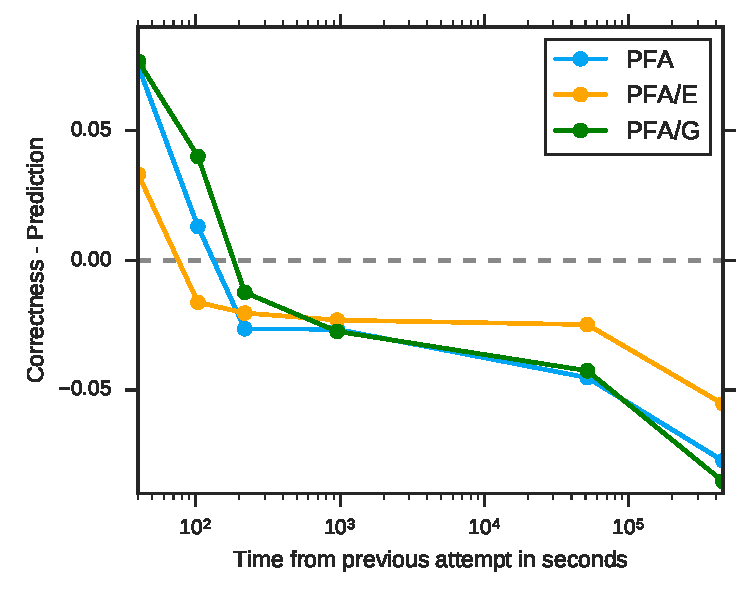
\includegraphics[width=\textwidth]{img/calibration-time-effect-off}
    \caption{}
    \label{fig:calibration-time-effect-off}
  \end{subfigure}
  \begin{subfigure}{.49\textwidth}
    \centering
    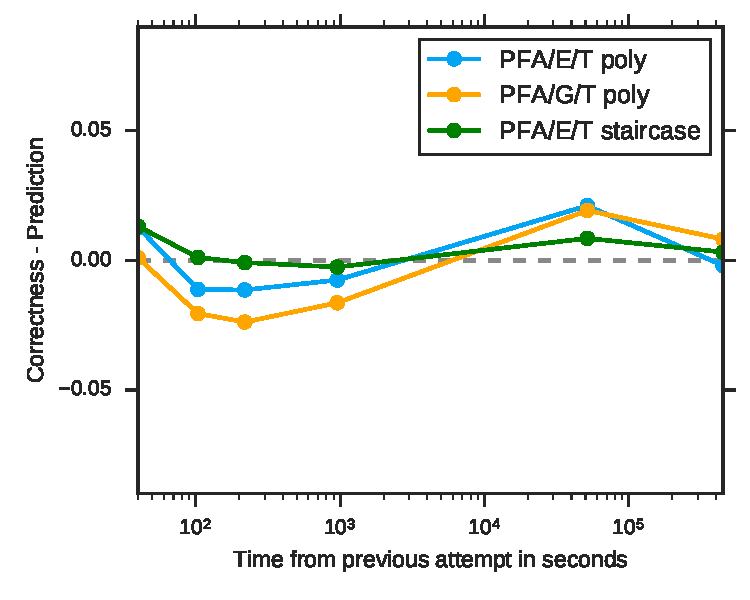
\includegraphics[width=\textwidth]{img/calibration-time-effect-on}
    \caption{}
    \label{fig:calibration-time-effect-on}
  \end{subfigure}
  \caption{Visualization of calibrations for the baseline models (left) and their extended versions with selected time effect functions (right). We learned the parameters of the staircase function from data as was described in chapter~\ref{staircase-function}, both power functions were estimated using the hill climbing method.}
  \label{fig:calibration1}
\end{figure}

Figure~\ref{fig:calibration2} shows calibration of all three time effect functions used in our experiments. The parameters of both models are summarized in Table~\ref{table:calibration2-parameters}. The analysis also suggests that the exponential function is not a very good choice as a time effect function for both models while the most calibrated models can be achieved with the power function.

\begin{table}
  \centering
  \caption{Parameters of calibrated models.}
  \begin{tabular}{ p{2cm}p{1cm}
                   S[table-format=1.3]S[table-format=1.3]
                   S[table-format=1.3]S[table-format=1.3]
                   S[table-format=1.3]S[table-format=1.3] }
   \toprule[\heavyrulewidth]
   & & \multicolumn{6}{c}{Time Effect Function} \\
   \cmidrule(r){3-8}
   &
   & \multicolumn{2}{c}{$f_{\mathit{log}}$}
   & \multicolumn{2}{c}{$f_{\mathit{exp}}$}
   & \multicolumn{2}{c}{$f_{\mathit{pow}}$} \\
   \cmidrule(r){3-8}
   &
   & \multicolumn{1}{c}{$a$}
   & \multicolumn{1}{c}{$c$}
   & \multicolumn{1}{c}{$a$}
   & \multicolumn{1}{c}{$c$}
   & \multicolumn{1}{c}{$a$}
   & \multicolumn{1}{c}{$c$} \\
   \midrule[\heavyrulewidth]
   \textbf{PFA/E/T} & &
     1.802 & 0.119 & 1.642 & 0.011 & 2.507 & 0.166 \\
   \midrule
   \multirow{2}{4em}{\textbf{PFA/G/T}} & $f_{\mathit{succ}}$ &
     1.669 & 0.102 & 0.96 & 0.002 & 3.138 & 0.198 \\
   & $f_{\mathit{fail}}$ &
     0.914 & 0.097 & 0.508 & 0.057 & 5.068 & 0.764 \\
   \bottomrule[\heavyrulewidth]
  \end{tabular}
  \label{table:calibration2-parameters}
\end{table}

\begin{figure}[htbp]
  \centering
  \begin{subfigure}{.49\textwidth}
    \centering
    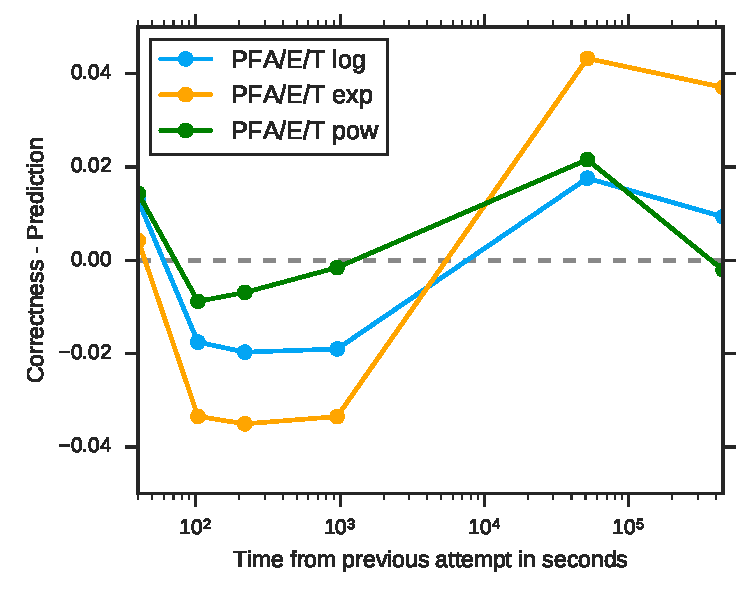
\includegraphics[width=\textwidth]{img/calibration-pfaet}
    \caption{}
    \label{fig:calibration-pfaet}
  \end{subfigure}
  \begin{subfigure}{.49\textwidth}
    \centering
    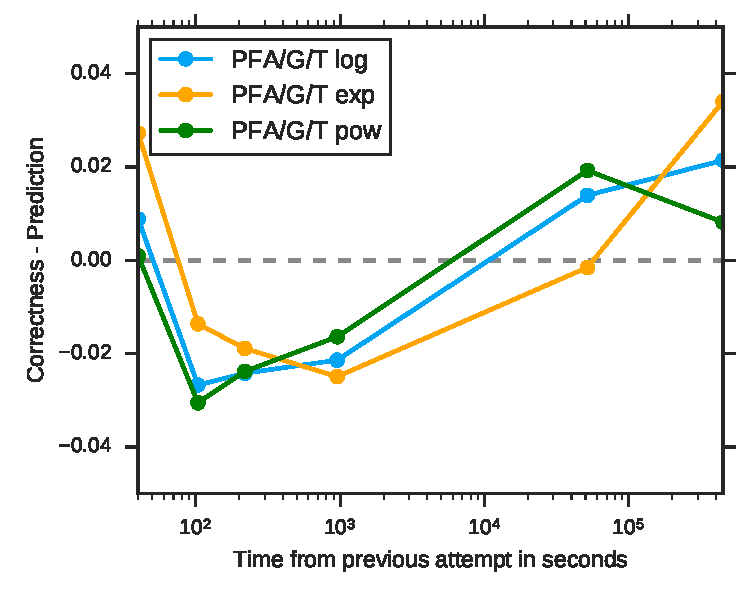
\includegraphics[width=\textwidth]{img/calibration-pfagt}
    \caption{}
    \label{fig:calibration-pfagt}
  \end{subfigure}
  \caption{Calibration analysis for (a) the PFA/E/T model and (b) the PFA/G/model with three time effect functions used in our experiments.}
  \label{fig:calibration2}
\end{figure}

\section{Evaluation}
\label{evaluation}

We evaluated the models on several different sets of data, including answers of all students, African and European countries, USA states, Czech rivers, world mountains and lakes. Parameters of all PFA-based models were estimated by running either hill climbing or the adjusted gradient descent. In all our experiments we used Elo model for the estimation of prior knowledge, where we estimated the parameters $\alpha$ and $\beta$ using grid search algorithm. On account of the quantification of model's performance we use several previously mentioned metrics, namely RMSE, LL, AUC and Accuracy (although the use of accuracy is not very suitable in our case as we discussed in chapter~\ref{metrics}).

\subsection{All Answers}

We compare the performance of all evaluated variations of examined models on a data set containing 150 thousand answers. We summarized the results in Table~\ref{table:results-all-answers} where we report on the estimated parameters and the scores of each used metric function.

It is clear that the models based on PFA/E perform best, although the improvement is not huge. The performance of the PFA/E/T model with all compared time effect functions is very similar, however, the staircase offers the best performance with RMSE $3.402$. Both the PFA/E model and the PFA/G model outperform the PFA/G/T model which uses a time effect function for penalizing old trials, nevertheless the difference is very small and the PFA/G/T model still shows significant improvement over the standard PFA model. Compared with the PFA/E model, there is also a small increase in performance of the PFA/E/RT model.

The improvement of models which account for ages of past trials may be more visible when we evaluate the performance on items where the last trial was practiced at more distant time. Table~\ref{table:results-all-answers-last-older} shows performance of all models evaluated only on answers where the last practice is older than 6~hours. In contrast, Table~\ref{table:results-all-answers-last-newer} shows the opposite, i.e. considered are answers where the last practice was performed at most 6~hours ago. The results show that the PFA/G/T model outperforms the PFA/G model in cases where the last trials are older (e.g. older then 6~hours).

\begin{table}
  \centering
  \caption{Performance of all variations of models focused on timing information of students' answers. The upper part of the table contains estimated parameters of each model. The lower part consists of scores for each metric. The best score overall is marked bold.}
  \sisetup{detect-weight=true,detect-inline-weight=math}
  \begin{tabular}{ p{2cm} l
                   S[table-format=1.4] S[table-format=1.4]
                   S[table-format=1.4] S[table-format=1.4] }
   \toprule[\heavyrulewidth]
   \toprule[\heavyrulewidth]
   & \multicolumn{1}{c}{Time Effect Fun.} & \multicolumn{4}{c}{Parameters} \\
   \midrule[\heavyrulewidth]
   & & \multicolumn{1}{c}{$\gamma$}
     & \multicolumn{1}{c}{$\delta$}
     & \multicolumn{1}{c}{$\xi$} & \\
   \cmidrule(r){3-6}
   \textbf{PFA}                & &  1.022 & -0.081 &        & \\
   \textbf{PFA/E}              & &  2.614 & -0.642 &        & \\
   \textbf{PFA/G}              & &  1.798 &  0.091 &  0.425 & \\
   \textbf{PFA/E/RT}           & &  1.453 & -1.356 &        & \\
   \midrule
   & & \multicolumn{1}{c}{$\gamma$}
     & \multicolumn{1}{c}{$\delta$}
     & \multicolumn{1}{c}{$a$}
     & \multicolumn{1}{c}{$c$} \\
   \cmidrule(r){3-6}
   \multirow{4}{4em}{\textbf{PFA/E/T}}
    & $f_{\mathit{pow}}$       &  2.004 & -0.713 &  2.931 &  0.27  \\
    & $f_{\mathit{log}}$       &  1.906 & -0.806 &  1.789 &  0.128 \\
    & $f_{\mathit{exp}}$       &  2.006 & -0.757 &  1.005 &  0.009 \\
    & $f_{\mathit{staircase}}$ &  1.814 & -0.827 &        &        \\
   \midrule
   & & \multicolumn{1}{c}{$a_{\mathit{succ}}$}
     & \multicolumn{1}{c}{$c_{\mathit{succ}}$}
     & \multicolumn{1}{c}{$a_{\mathit{fail}}$}
     & \multicolumn{1}{c}{$c_{\mathit{fail}}$} \\
   \cmidrule(r){3-6}
   \multirow{3}{3em}{\textbf{PFA/G/T}}
    & $f_{\mathit{pow}}$       &  3.138 &  0.198 &  5.068 &  0.764 \\
    & $f_{\mathit{log}}$       &  1.669 &  0.102 &  0.914 &  0.097 \\
    & $f_{\mathit{exp}}$       &  0.96  &  0.002 &  0.508 &  0.057 \\
   \midrule[\heavyrulewidth]
   \midrule[\heavyrulewidth]
   & \multicolumn{1}{c}{Time Effect Fun.}
   & \multicolumn{1}{c}{RMSE}
   & \multicolumn{1}{c}{AUC}
   & \multicolumn{1}{c}{\textsc{Acc}}
   & \multicolumn{1}{c}{LL} \\
   \midrule[\heavyrulewidth]
   \textbf{PFA}      & &  0.3651 & 0.753 
     & 0.822 & \multicolumn{1}{S[table-format=5]}{-75215} \\
   \textbf{PFA/E}    & &  0.3456 & 0.8
     & 0.836 & \multicolumn{1}{S[table-format=5]}{-55503} \\
   \textbf{PFA/G}    & &  0.35   & 0.782
     & 0.836 & \multicolumn{1}{S[table-format=5]}{-58420} \\
   \textbf{PFA/E/RT} & &  0.3449 & 0.799
     & 0.836 & \multicolumn{1}{S[table-format=5]}{-55436} \\
   \midrule
   \multirow{4}{4em}{\textbf{PFA/E/T}}
     & $f_{\mathit{pow}}$       &  0.3406 & 0.806 & \bfseries 0.841
     & \multicolumn{1}{S[table-format=5]}{-54082} \\
     & $f_{\mathit{log}}$       &  0.3407 & 0.806 & 0.84
     & \multicolumn{1}{S[table-format=5]}{-54088} \\
     & $f_{\mathit{exp}}$       &  0.341  & \bfseries 0.808 & \bfseries 0.841
     & \multicolumn{1}{S[table-format=5]}{-54145} \\
     & $f_{\mathit{staircase}}$ & \bfseries 0.3402 & 0.807 & \bfseries 0.841
     & \multicolumn{1}{S[table-format=5]}{\bfseries -54030} \\
   \midrule
   \multirow{3}{3em}{\textbf{PFA/G/T}}
     & $f_{\mathit{pow}}$       &  0.3493 & 0.783 & 0.834
     & \multicolumn{1}{S[table-format=5]}{-60128} \\
     & $f_{\mathit{log}}$       &  0.3516 & 0.775 & 0.834
     & \multicolumn{1}{S[table-format=5]}{-63084} \\
     & $f_{\mathit{exp}}$       &  0.3508 & 0.775 & 0.834
     & \multicolumn{1}{S[table-format=5]}{-61882} \\
   \bottomrule[\heavyrulewidth]
   \bottomrule[\heavyrulewidth]
  \end{tabular}
  \label{table:results-all-answers}
\end{table}

\begin{table}
  \centering
  \caption{Performance of models when we consider only answers where the last trial is older than 6~hours.}
  \sisetup{detect-weight=true,detect-inline-weight=math}
  \begin{tabular}{ p{2cm} l
                   S[table-format=1.4] S[table-format=1.4]
                   S[table-format=1.4] S[table-format=1.4] }
   \toprule[\heavyrulewidth]
   \toprule[\heavyrulewidth]
   & \multicolumn{1}{c}{Time Effect Fun.} & \multicolumn{4}{c}{Metric} \\
   \midrule[\heavyrulewidth]
   &
   & \multicolumn{1}{c}{RMSE}
   & \multicolumn{1}{c}{AUC}
   & \multicolumn{1}{c}{\textsc{Acc}}
   & \multicolumn{1}{c}{LL} \\
   \midrule[\heavyrulewidth]
   \textbf{PFA}      & &  0.3665 & 0.727 & 0.831
     & \multicolumn{1}{S[table-format=5]}{-16120} \\
   \textbf{PFA/E}    & &  0.3491 & 0.752 & 0.84
     & \multicolumn{1}{S[table-format=5]}{-10575} \\
   \textbf{PFA/G}    & &  0.357  & 0.754 & 0.84
     & \multicolumn{1}{S[table-format=5]}{-11783} \\
   \textbf{PFA/E/RT} & &  0.3487 & 0.768 & 0.841
     & \multicolumn{1}{S[table-format=5]}{-11308} \\
   \midrule
   \multirow{4}{4em}{\textbf{PFA/E/T}}
     & $f_{\mathit{pow}}$       &  \bfseries 0.3417 & 0.777 & \bfseries 0.842
     & \multicolumn{1}{S[table-format=5]}{-10056} \\
     & $f_{\mathit{log}}$       &  0.342  & \bfseries 0.779 & 0.84
     & \multicolumn{1}{S[table-format=5]}{-10061} \\
     & $f_{\mathit{exp}}$       &  0.3433 & 0.776 & 0.84
     & \multicolumn{1}{S[table-format=5]}{-10142} \\
     & $f_{\mathit{staircase}}$ &  0.3418 & 0.778 & \bfseries 0.842
     & \multicolumn{1}{S[table-format=5]}{\bfseries -10045} \\
   \midrule
   \multirow{3}{3em}{\textbf{PFA/G/T}}
     & $f_{\mathit{pow}}$       &  0.3516 & 0.755 & 0.84
     & \multicolumn{1}{S[table-format=5]}{-10677} \\
     & $f_{\mathit{log}}$       &  0.3524 & 0.771 & 0.841
     & \multicolumn{1}{S[table-format=5]}{-10924} \\
     & $f_{\mathit{exp}}$       &  0.3521 & 0.75  & 0.841
     & \multicolumn{1}{S[table-format=5]}{-10939} \\
   \bottomrule[\heavyrulewidth]
   \bottomrule[\heavyrulewidth]
  \end{tabular}
  \label{table:results-all-answers-last-older}
\end{table}

\begin{table}
  \centering
  \caption{Performance of models when we consider only answers where the last trial was performed at most 6~hours ago.}
  \sisetup{detect-weight=true,detect-inline-weight=math}
  \begin{tabular}{ p{2cm} l
                   S[table-format=1.4] S[table-format=1.4]
                   S[table-format=1.4] S[table-format=1.4] }
   \toprule[\heavyrulewidth]
   \toprule[\heavyrulewidth]
   & \multicolumn{1}{c}{Time Effect Fun.} & \multicolumn{4}{c}{Metric} \\
   \midrule[\heavyrulewidth]
   &
   & \multicolumn{1}{c}{RMSE}
   & \multicolumn{1}{c}{AUC}
   & \multicolumn{1}{c}{\textsc{Acc}}
   & \multicolumn{1}{c}{LL} \\
   \midrule[\heavyrulewidth]
   \textbf{PFA}      & &  0.3544 & 0.733 & 0.832
     & \multicolumn{1}{S[table-format=5]}{-43559} \\
   \textbf{PFA/E}    & &  0.3367 & 0.786 & 0.842
     & \multicolumn{1}{S[table-format=5]}{-31062} \\
   \textbf{PFA/G}    & &  0.3411 & 0.766 & 0.842
     & \multicolumn{1}{S[table-format=5]}{-32776} \\
   \textbf{PFA/E/RT} & &  0.3368 & 0.785 & 0.84
     & \multicolumn{1}{S[table-format=5]}{-32161} \\
   \midrule
   \multirow{4}{4em}{\textbf{PFA/E/T}}
     & $f_{\mathit{pow}}$       &  \bfseries 0.3303 & 0.784 & \bfseries 0.852
     & \multicolumn{1}{S[table-format=5]}{-30160} \\
     & $f_{\mathit{log}}$       &  \bfseries 0.3303 & 0.784 & 0.851
     & \multicolumn{1}{S[table-format=5]}{-30161} \\
     & $f_{\mathit{exp}}$       &  0.3305 & \bfseries 0.787 & 0.849
     & \multicolumn{1}{S[table-format=5]}{\bfseries -30137} \\
     & $f_{\mathit{staircase}}$ &  0.3305 & 0.784 & 0.85
     & \multicolumn{1}{S[table-format=5]}{-30178} \\
   \midrule
   \multirow{3}{3em}{\textbf{PFA/G/T}}
     & $f_{\mathit{pow}}$       &  0.3423 & 0.756 & 0.842
     & \multicolumn{1}{S[table-format=5]}{-35584} \\
     & $f_{\mathit{log}}$       &  0.346  & 0.741 & 0.844
     & \multicolumn{1}{S[table-format=5]}{-38293} \\
     & $f_{\mathit{exp}}$       &  0.3447 & 0.74  & 0.843
     & \multicolumn{1}{S[table-format=5]}{-37076} \\
   \bottomrule[\heavyrulewidth]
   \bottomrule[\heavyrulewidth]
  \end{tabular}
  \label{table:results-all-answers-last-newer}
\end{table}

\subsection{Countries and USA States}

Most answers in our data set are from the citizens of the Czech Republic, i.e. Europeans, who generally have much better knowledge of the countries in Europe than for example the countries in Africa. Very important aspect of learning the locations of individual places is their context. It is way easier to encode and retain the locations that are neighbors with an already known place.

\begin{figure}[htbp]
  \centering
  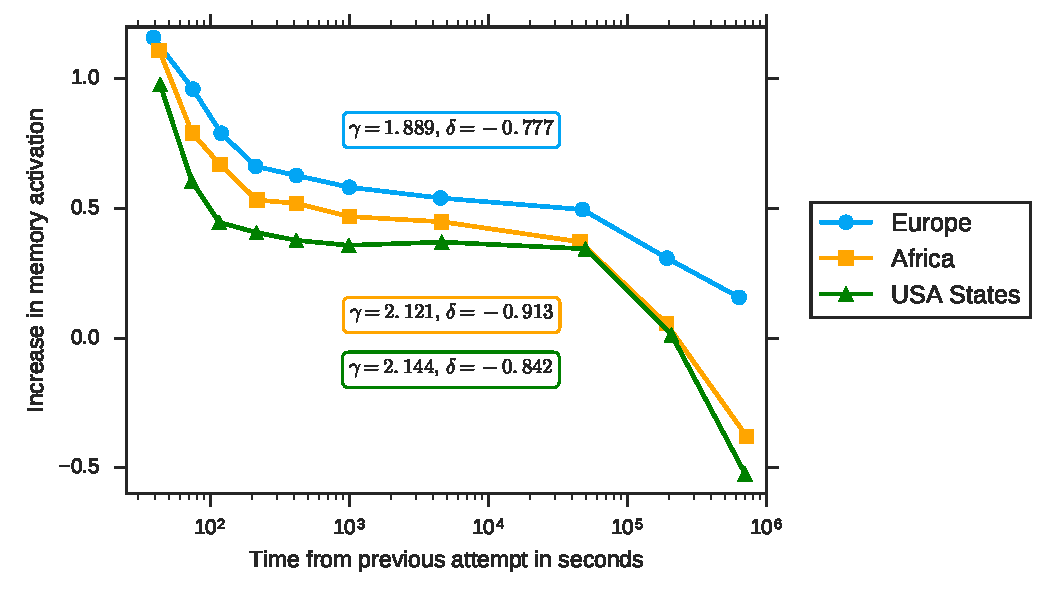
\includegraphics[width=\textwidth]{img/africa-europe-usa-states}
  \caption{Learned values of the staircase function for African countries, European countries and USA states.}
  \label{fig:africa-europe-usa-states}
\end{figure}

In Figure~\ref{fig:africa-europe-usa-states} we observe the differences between learned values of the staircase function when the data set is separated in three by the type of place---African countries, European countries and USA states. The learned values suggest that the rate of forgetting (or more precisely the change in memory activation) is very similar in all examined types of places when the timing distance between current and the last practice is lower than one day, however, the African countries and USA states are forgotten faster after longer periods of time.

TODO: table comparing all models.

\subsection{Mountains, Rivers and Lakes}

Another interesting question how the number of facts affects easiness of learning, since intuitively it's easier to learn all facts from domains of small sizes. We divided the data set into three, containing only the answers to questions about either 21 lakes, 71 mountains or 84 rivers. The result of learned parameters of $\gamma$, $\delta$ and the staircase function is shown on Figure~\ref{fig:lakes-rivers-mountains}.

\begin{figure}[htbp]
  \centering
  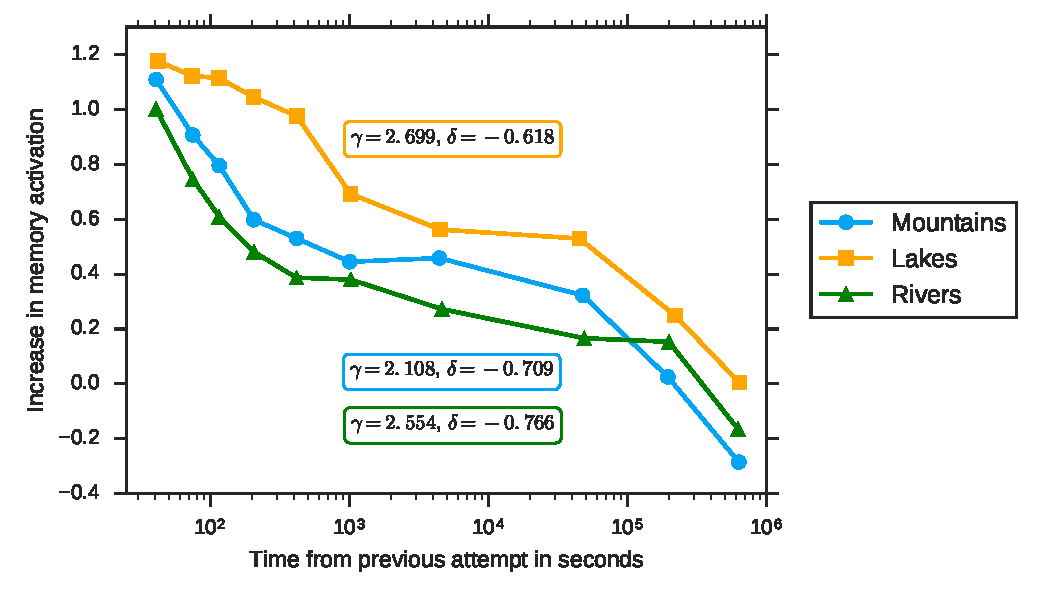
\includegraphics[width=\textwidth]{img/lakes-rivers-mountains}
  \caption{Learned values of the staircase function from data sets containing only rivers, lakes and mountains.}
  \label{fig:lakes-rivers-mountains}
\end{figure}

TODO: table comparing all models.

\section{Further Analysis}
\label{further-analysis}

\subsection{At School vs At Home}

An interesting question is how much students' motivation affects the speed of learning or the rate of forgetting. Figure~\ref{fig:at-home-vs-at-school} shows the learned parameters of a staircase function on two different data sets. The first data set labeled as ``At School'' contained only the answers from groups of 10 or more students with the same IP address (the assumption is that these students practice geography in classrooms). The second data set labeled as ``At Home'' contained all the other answers of students.

\begin{figure}[htbp]
  \centering
  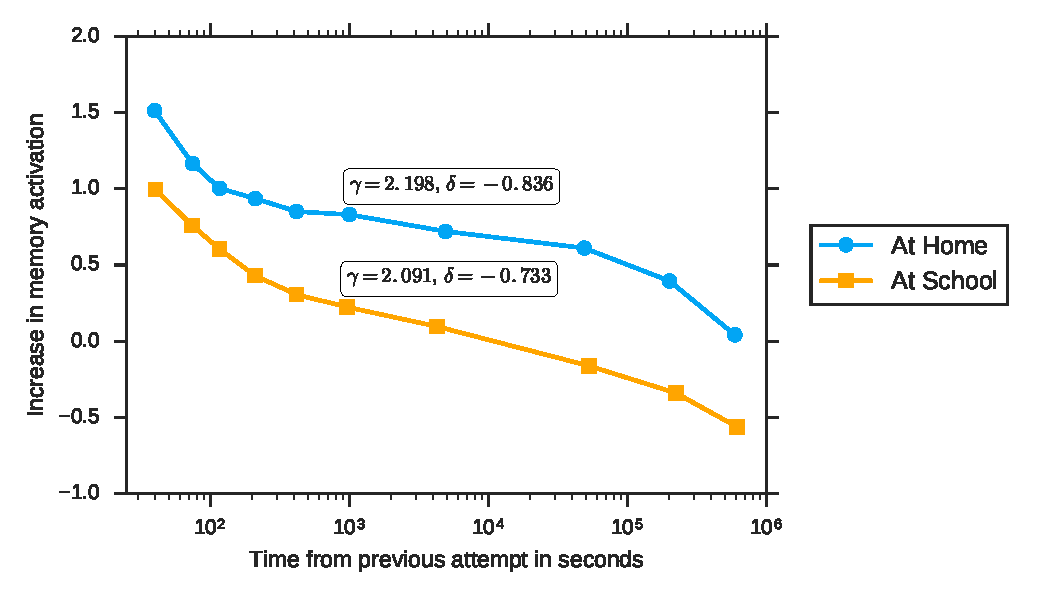
\includegraphics[width=\textwidth]{img/at-home-vs-at-school}
  \caption{Comparison of students who practice geography at school (i.e. in classrooms) and students who practice at home (i.e. on their own initiative).}
  \label{fig:at-home-vs-at-school}
\end{figure}

The learned values of the staircase function and the parameters $\gamma$, $\delta$ indicate that students who practice geography at school learn indeed slower and forget the learned material faster then the students who are motivated by some other means. Note that the difference in the rate of forgetting between both types of students may be caused by teaching methods (more material is learned in shorter periods of time). Since the system we analyze is adaptive and selects questions based on student's knowledge, we believe this is not the only cause.
